\documentclass[tikz, border=10pt]{standalone}

\usepackage{tikz}
\usetikzlibrary{shapes.geometric, arrows.meta, positioning, fit, backgrounds, calc}

% ── Colours ──────────────────────────────────────────────────────────
\definecolor{laneuser}{RGB}{220,235,255}
\definecolor{laneback}{RGB}{220,245,230}
\definecolor{lanellm}{RGB}{255,235,210}
\definecolor{taskblue}{RGB}{70,130,180}
\definecolor{taskgreen}{RGB}{60,160,100}
\definecolor{taskorange}{RGB}{200,110,40}
\definecolor{gatecolor}{RGB}{230,180,40}
\definecolor{labelgray}{RGB}{80,80,90}

% ── Node styles ───────────────────────────────────────────────────────
\tikzset{
  task/.style={
    rectangle, rounded corners=4pt,
    minimum width=2.6cm, minimum height=0.8cm,
    draw=#1!80!black, fill=#1!20,
    font=\scriptsize\bfseries, text centered, align=center,
    text width=2.4cm
  },
  gateway/.style={
    diamond, aspect=1.6,
    minimum width=2.2cm, minimum height=0.75cm,
    draw=gatecolor!80!black, fill=gatecolor!25,
    font=\scriptsize, text centered, align=center,
    inner sep=1pt
  },
  startevent/.style={
    circle, minimum size=0.55cm,
    draw=taskgreen!80!black, fill=taskgreen!30,
    line width=1.2pt
  },
  endevent/.style={
    circle, minimum size=0.55cm,
    draw=taskblue!80!black, fill=taskblue!30,
    line width=2.5pt
  },
  flow/.style={-Stealth, thick, color=labelgray},
  laneheader/.style={
    rectangle, minimum width=1.1cm,
    draw=gray!50, fill=gray!15,
    font=\small\bfseries, rotate=90,
    text centered, align=center
  }
}

\begin{document}
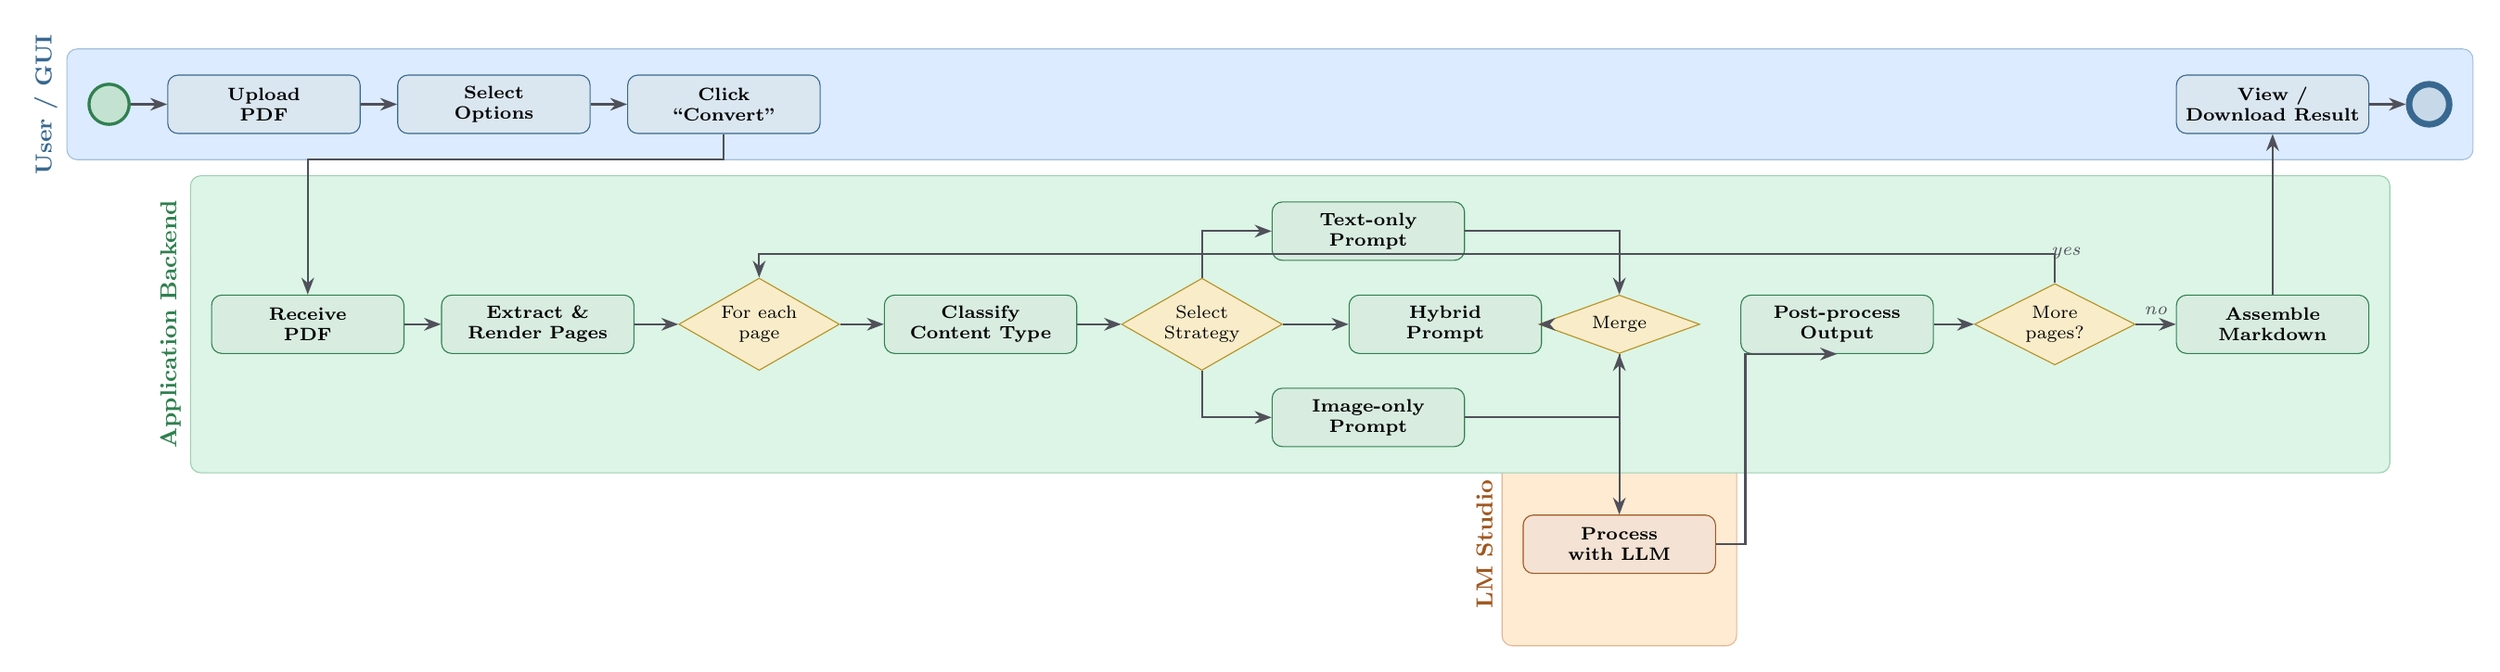
\begin{tikzpicture}[node distance=0.55cm and 0.5cm]

% ═══════════════════════════════════════════════════════════════════
% LANE 1 — USER / GUI  (top)
% ═══════════════════════════════════════════════════════════════════

\node[startevent] (start) {};

\node[task=taskblue, right=0.5cm of start]
  (upload) {Upload\\PDF};

\node[task=taskblue, right=0.5cm of upload]
  (options) {Select\\Options};

\node[task=taskblue, right=0.5cm of options]
  (convert) {Click\\``Convert''};

% ── spacer so backend nodes align nicely below ───────────────────
\coordinate (drop1) at ($(convert.south)+(0,-0.55)$);

% ═══════════════════════════════════════════════════════════════════
% LANE 2 — APPLICATION BACKEND  (middle)
% ═══════════════════════════════════════════════════════════════════

\node[task=taskgreen,
      below=2.2cm of upload,
      xshift=0.6cm]
  (receive) {Receive\\PDF};

\node[task=taskgreen, right=0.5cm of receive]
  (extract) {Extract \&\\Render Pages};

\node[gateway, right=0.6cm of extract]
  (pageloop) {For each\\page};

\node[task=taskgreen, right=0.6cm of pageloop]
  (classify) {Classify\\Content Type};

\node[gateway, right=0.6cm of classify]
  (stratgate) {Select\\Strategy};

% ── three strategy branches ──────────────────────────────────────
\node[task=taskgreen,
      above right=0.55cm and 0.4cm of stratgate]
  (sttext)  {Text-only\\Prompt};

\node[task=taskgreen,
      right=0.9cm of stratgate]
  (sthybrid){Hybrid\\Prompt};

\node[task=taskgreen,
      below right=0.55cm and 0.4cm of stratgate]
  (stimage) {Image-only\\Prompt};

% ── merge after strategies ───────────────────────────────────────
\node[gateway,
      right=3.5cm of stratgate]
  (merge) {Merge};

% ═══════════════════════════════════════════════════════════════════
% LANE 3 — LM STUDIO  (lower middle)
% ═══════════════════════════════════════════════════════════════════

\node[task=taskorange,
      below=2.2cm of merge]
  (llmproc) {Process\\with LLM};

% ═══════════════════════════════════════════════════════════════════
% LANE 2 continued — post-processing
% ═══════════════════════════════════════════════════════════════════

\node[task=taskgreen,
      right=0.55cm of merge]
  (postproc){Post-process\\Output};

\node[gateway, right=0.55cm of postproc]
  (morepages){More\\pages?};

\node[task=taskgreen, right=0.55cm of morepages]
  (assemble){Assemble\\Markdown};

% ═══════════════════════════════════════════════════════════════════
% LANE 1 continued — result display
% ═══════════════════════════════════════════════════════════════════

\node[task=taskblue,
      above=2.2cm of assemble]
  (display) {View /\\Download Result};

\node[endevent, right=0.5cm of display] (end) {};

% ═══════════════════════════════════════════════════════════════════
% SEQUENCE FLOWS
% ═══════════════════════════════════════════════════════════════════

% User lane
\draw[flow] (start)   -- (upload);
\draw[flow] (upload)  -- (options);
\draw[flow] (options) -- (convert);
\draw[flow] (display) -- (end);

% User → Backend handoff
\draw[flow] (convert.south)
  -- ++(0,-0.35)
  -| (receive.north);

% Backend pipeline
\draw[flow] (receive)   -- (extract);
\draw[flow] (extract)   -- (pageloop);
\draw[flow] (pageloop)  -- (classify);
\draw[flow] (classify)  -- (stratgate);

% Strategy branches
\draw[flow] (stratgate.north) |- (sttext.west);
\draw[flow] (stratgate.east)  -- (sthybrid.west);
\draw[flow] (stratgate.south) |- (stimage.west);

% Merge strategies
\draw[flow] (sttext.east)  -| (merge.north);
\draw[flow] (sthybrid.east) -- (merge.west);
\draw[flow] (stimage.east) -| (merge.south);

% Backend → LM Studio handoff
\draw[flow] (merge.south)
  -- ++(0,-0.4)
  -- (llmproc.north);

% LM Studio → Backend handoff
\draw[flow] (llmproc.east)
  -- ++(0.4,0)
  |- (postproc.south);

% Post-processing pipeline
\draw[flow] (postproc) -- (morepages);

% More pages loop back
\draw[flow] (morepages.north)
  -- ++(0, 0.4)
  node[above, font=\scriptsize\itshape, midway, xshift=0.15cm] {yes}
  -| (pageloop.north);

% No more pages → assemble
\draw[flow] (morepages) -- node[above, font=\scriptsize\itshape]{no} (assemble);

% Backend → User handoff
\draw[flow] (assemble.north)
  -- ++(0, 0.35)
  -| (display.south);

% ═══════════════════════════════════════════════════════════════════
% SWIM LANE BACKGROUNDS
% ═══════════════════════════════════════════════════════════════════
\begin{pgfonlayer}{background}

  % Lane 1 — User / GUI
  \node[rectangle,
        draw=taskblue!50, fill=laneuser, rounded corners=4pt,
        fit=(start)(upload)(options)(convert)(display)(end),
        inner xsep=8pt, inner ysep=10pt,
        label={[font=\small\bfseries, text=taskblue!80!black,
                rotate=90, anchor=south]left:User / GUI}]
    (lane1) {};

  % Lane 3 — LM Studio (drawn before lane 2 so lane 2 overlaps it)
  \node[rectangle,
        draw=taskorange!50, fill=lanellm, rounded corners=4pt,
        fit=(llmproc),
        inner xsep=8pt, inner ysep=28pt,
        label={[font=\small\bfseries, text=taskorange!80!black,
                rotate=90, anchor=south]left:LM Studio}]
    (lane3) {};

  % Lane 2 — Application Backend
  \node[rectangle,
        draw=taskgreen!50, fill=laneback, rounded corners=4pt,
        fit=(receive)(extract)(pageloop)(classify)(stratgate)
            (sttext)(sthybrid)(stimage)(merge)(postproc)(morepages)(assemble),
        inner xsep=8pt, inner ysep=10pt,
        label={[font=\small\bfseries, text=taskgreen!80!black,
                rotate=90, anchor=south]left:Application Backend}]
    (lane2) {};

\end{pgfonlayer}

\end{tikzpicture}
\end{document}
